\chapter{Resultados y discusión}

La esencia de esta tesis es desarrollar un programa de cómputo científico para explorar la posible aplicación del análisis multifractal en estructuras proteicas. Este programa podría ser una herramienta útil para caracterizar las distintas etapas del plegamiento proteico, describiéndolas en términos de la dinámica de formación de agregados estructurales, lo que permitiría una comprensión más profunda de estos procesos. En consecuencia, es necesaria una explicación detallada de todo esto. Por lo que he dividido esta descripción en dos secciones; el algoritmo y su uso para la obtención de resultados. 
 
 \clearpage
 
\section{Algoritmo (diseño del programa)}

 El procedimiento general del programa \textbf{\textit{molmassfractaldim}} se describe en el diagrama de flujo de la figura \ref{dfMolFractalDim}), cuyos pasos se explican a detalle en las siguientes subsecciones.
 
 
 \begin{figure}[h!]
 	\begin{center}
 		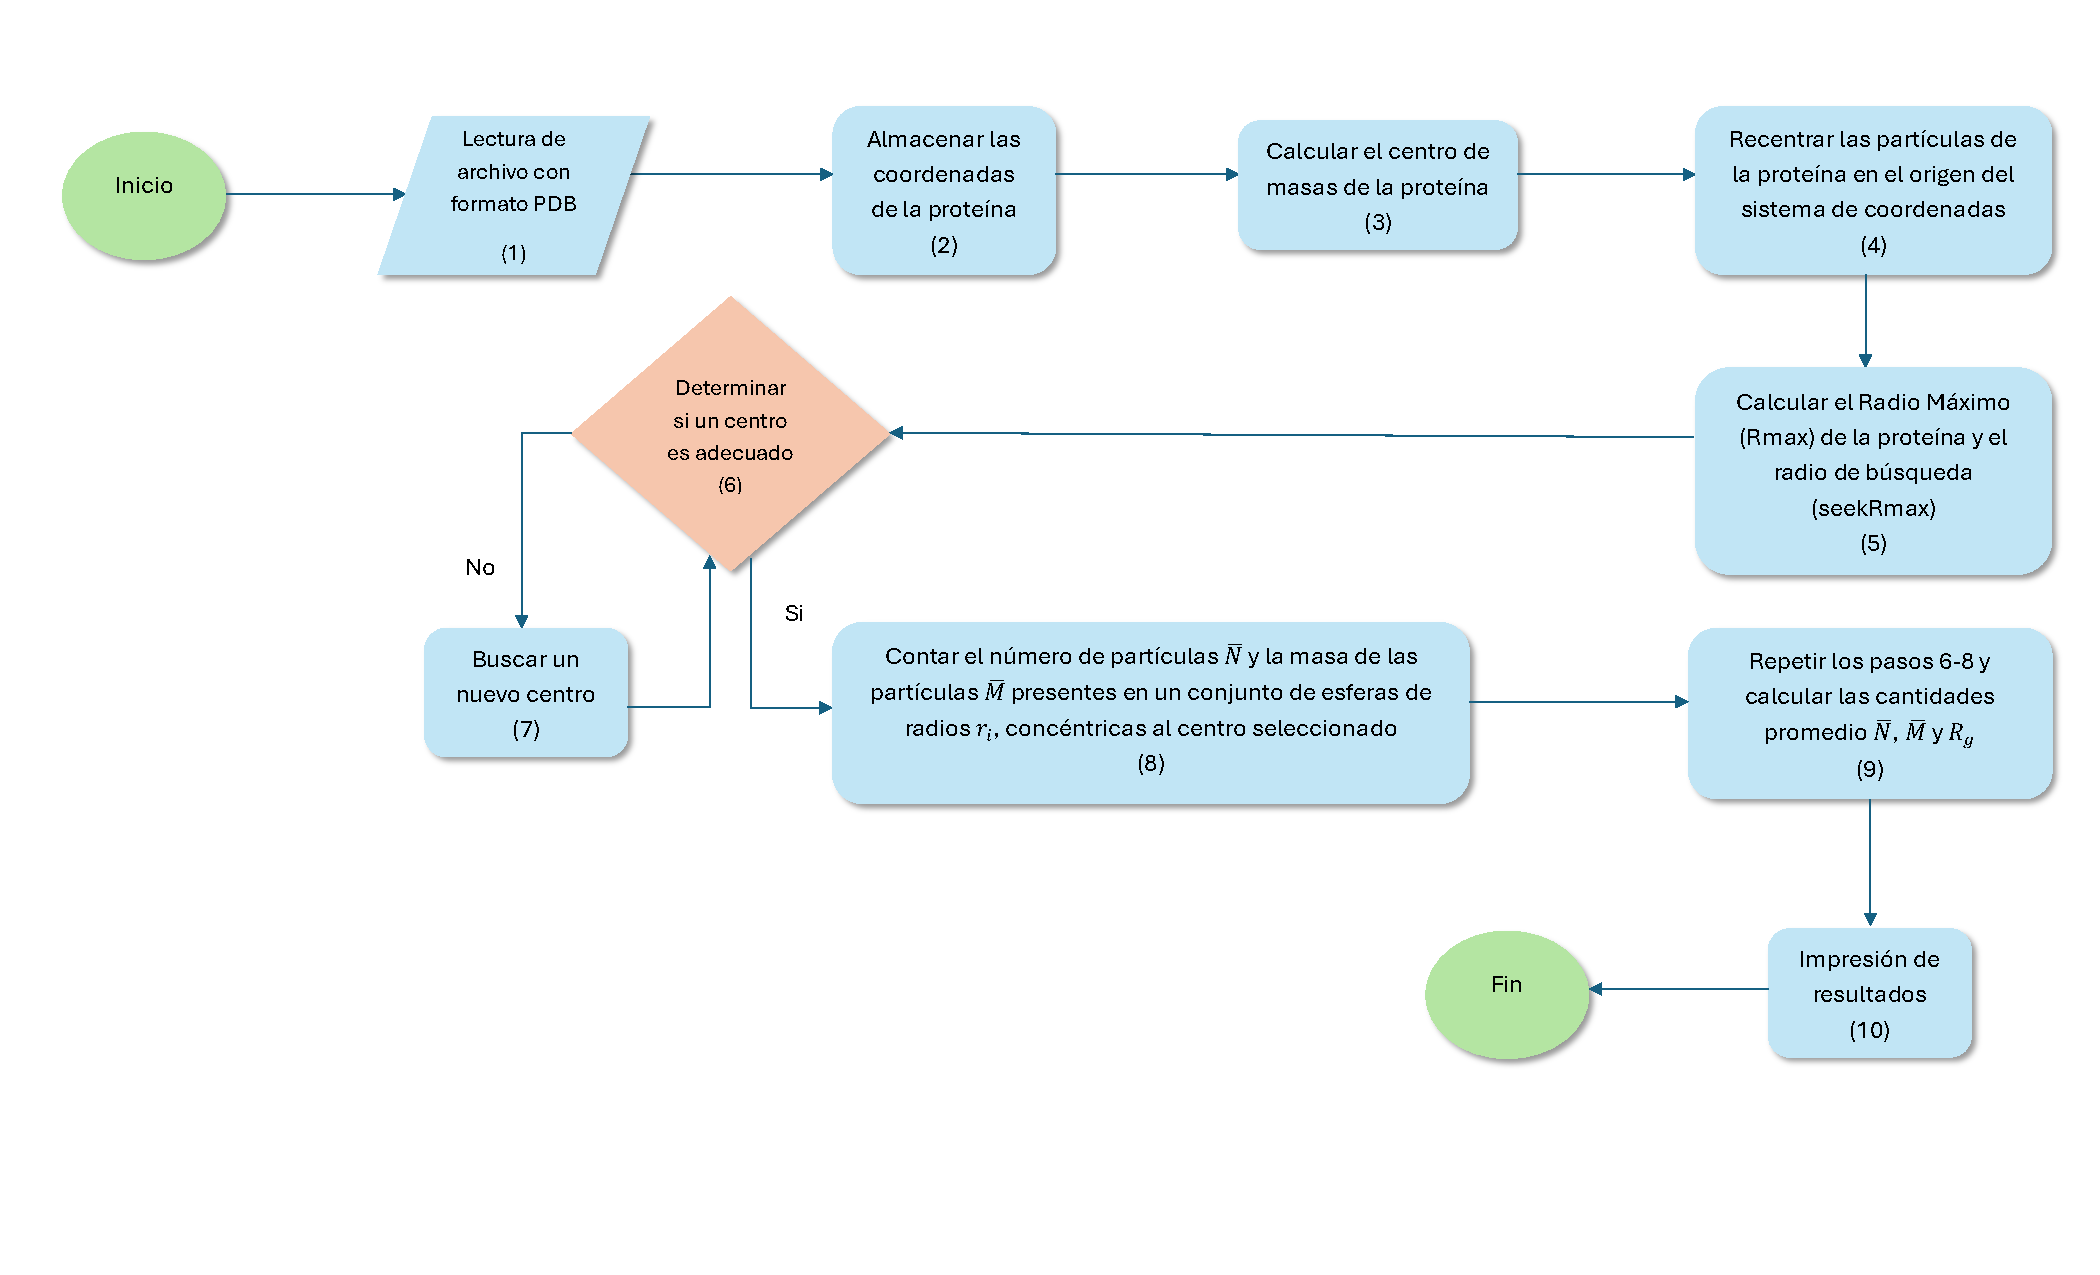
\includegraphics[width=\textwidth]{graphs/dfMolFractalDim}
 		\caption{Diagrama de flujo general del programa \textit{molmassfractaldim}.}
 		\label{dfMolFractalDim}
 	\end{center}
 \end{figure}
 

 
 \subsection {Pasos 1, 2, 3 y 4 del diagrama de flujo general}
 
	\begin{itemize}
		\item \textbf{Paso 1}:  El programa \textbf{\textit{molmassfractaldim}} inicia con el
		uso de una clase llamada \textit{InputMoleculePDB} que se encargar de realizar 
		la lectura de un archivo en formato \textit{PDB} que contiene datos 
		fundamentales para el programa como: 
		
		\begin{itemize}
			\item Número atómico y número de átomos presentes en la proteína.
			\item Las coordenadas átomicas del sistema expresada en $\textup{\r{A}}$ngstr\"oms.
		\end{itemize}
		
		\item \textbf{Paso 2}: Usa una clase llamada \textit{Molecule}
		que esta diseñada para representar a una molécula como un conjunto de 
		átomos. En este paso \textit{Molecule} se encarga de extraer y guardar las coordenas átomicas del sistema $(x, y, z)$.\\
		
		\item \textbf{Paso 3}: Nuevamente se usa la clase 
		\textit{Molecule} para el cálculo de propiedades moleculares como:
		
		\begin{itemize}
			\item Determinar la fórmula empírica de la molécula, contado la cantidad de átomos por número atómico.
			\item Devolver valores como la cantidad de átomos de un tipo específico 
			dado por el número átomico.
			\item Calcular los extremos mínimos y máximos de todos los átomos para definir 
			el radio máximo desde el origen de la esfera que envuelve a la proteína.
			\item Calcula el centro de masa considerando las masas atómicas.
			\item Calcula el centroide (promedio aritmético de las coordenadas de todos los
			átomos, sin considerar su masa).
		\end{itemize}
		
		Por último en este paso, la clase \textit{Molecule} también se encarga de trasladar la proteína de modo que su centroide coincida con el origen de las coordenas $(0, 0, 0)$.  
		
		
		\item \textbf{Paso 4}: En este paso la clase \textit{Molecule} se encarga de identificar enlaces covalentes entre átomos según la distancia que exista entre ellos y sus radios de Van Der Waals para devolver una lista con los índices de vecinos cercanos a un átomo dado.
		
	\end{itemize}


	\subsection{Paso 5 del diagrama de flujo general}
	
	En este paso una nueva clase llamada \textit{massfractaldim} determina el radio máximo de la proteína $R_{max}$, calculado como la distancia máxima desde el origen hasta cualquier átomo de la molécula. Matemáticamente esto se escribe como:
	
	\begin{equation}
		R_{max} = max_{i} \sqrt{x^{2}_{i} + y^{2}_{i} + z^{2}_{i}}
	\end{equation}
 	
 	Donde $x_{i}, y_{i}, z_{i}$ representan las coordenadas cartesianas de un conjunto de átomos en tres dimensiones.
 	
 	Hecho lo anterior, en esta misma clase se define un radio dentro del cual se buscan puntos de medición adecuados para analizar la distribución de masa. A este radio se le conoce como $seekRmax$ que a través de un condicional de tipo \textit{if} se asegura que el valor de \textit{seekRmax} tenga un valor por defecto de $75\%$ tamaño del clúster. Otros usos que tiene \textit{seekRmax} son:
 	
 	\begin{itemize}
 		\item Se asegura de que los puntos de medición no estén demasiado cerca de los límites del clúster.
 		\item Evita que los círculos de medición se salgan del clúster del átomos. 
 		\item Evita tomar semillas demasiado cerca de los bordes del clúster.
 	\end{itemize}
 
 	A continuación se calculan los incrementos de radio
 	
 	Se prepara un vector de resultados 
 	
 
 
 
 
 
 
 
 
 
 

El propósito principal del programa \textit{molmassfractaldim} es determinar la dimesi\'{o}n fractal de masa mediante la caracterizaci\'{o}n de la geometría interna de un sistema proteico. Esto se logra construyendo una tabla de \(r_i\), \( \bar{N}(r_i)\) y \( \bar{M}(r_i)\), donde;

\begin{itemize}
	\item \(r_i\) es el radio de medida centrado en posiciones aleatorias de una prote\'{i}na con valores m\'{i}nimos y m\'{a}ximos definidos como \(mr_{min}\) y \(mr_{max}\).
	\item \( \bar{N}(r_i)\) es el número promedio de partículas contenidas dentro de un radio \(r_i\). 
	\item  \( \bar{M}(r_i)\) es el n\'{u}mero de masa promedio de las part\'{i}culas contenidas en el radio \(r_i\).
\end{itemize}








Posteriormente, los valores de \( \bar{N}(r_i) \) y \( \bar{M}(r_i)\) pueden analizarse mediante regresiones lineales para determinar la dimensi\'{o}n fractal de masa. Para calcular los valores de \(r_i\), \( \bar{N}(r_i)\) y \( \bar{M}(r_i)\), el algoritmo sigue los siguientes pasos:


\begin{enumerate}
	\item Inicializaci\'{o}n\\
	 Se carga un objeto llamado Molecule que contiene la informaci\'{o}n estructural del sistema (coordenadas y masas de los elementos presentes en la prote\'{i}na).
	
	\item Configuraci\'{o}n de par\'{a}metros\\
	Se calcula el centro de masas del cl\'{u}ster.\\
	Se recentran las part\'{i}culas de la prote\'{i}na en el origen del sistema de coordenadas.\\
	Se define el radio m\'{a}ximo del cluster \(R_{max}\) (la mayor distancia entre un \'{a}tomo y el origen).\\
	Se define el radio m\'{a}ximo de b\'{u}squeda de semillas como \(seekR_{max}\) para evitar que los c\'{i}rculos de medici\'{o}n se salgan del cl\'{u}ster.\\
	Se definen los radios m\'{i}nimo y m\'{a}ximo de medida como \(mr_{min}\) y \(mr_{max}\).\\
	Se calcula el n\'{u}mero de divisiones como \(nr\) y el incremento radial \(dr\).\\
	Se define el n\'{u}mero de medidas por centro como nMeas y el n\'{u}mero total de c\'{i}rculos a considerar.
	
	\item Generaci\'{o}n de puntos de medida\\
	Se eligen de manera aleatoria part\'{i}culas del sistema como centros de las circunferencias de medida. Para cada centro, se identifican las part\'{i}culas contenidas dentro del radio m\'{a}ximo (\(R_{max}\)).
	
	\item Acumulaci\'{o}n de datos\\
	Para cada radio \( r_i \), se cuenta cu\'{a}ntas part\'{i}culas est\'{a}n contenidas dentro de ese radio respecto al centro actual. Esta cuenta se repite para m\'{u}ltiples centros y se promedia para obtener \( \bar{N}(r_i) \).
	
	
	\item Salida de resultados\\
	Los vectores \(r_{i}\), \( \bar{N}(r_i) \) y \( \bar{M}(r_i)\) pueden visualizarse en pantalla o guardarse en un archivo externo.
\end{enumerate}




